% Options for packages loaded elsewhere
\PassOptionsToPackage{unicode}{hyperref}
\PassOptionsToPackage{hyphens}{url}
\documentclass[
]{book}
\usepackage{xcolor}
\usepackage{amsmath,amssymb}
\setcounter{secnumdepth}{5}
\usepackage{iftex}
\ifPDFTeX
  \usepackage[T1]{fontenc}
  \usepackage[utf8]{inputenc}
  \usepackage{textcomp} % provide euro and other symbols
\else % if luatex or xetex
  \usepackage{unicode-math} % this also loads fontspec
  \defaultfontfeatures{Scale=MatchLowercase}
  \defaultfontfeatures[\rmfamily]{Ligatures=TeX,Scale=1}
\fi
\usepackage{lmodern}
\ifPDFTeX\else
  % xetex/luatex font selection
\fi
% Use upquote if available, for straight quotes in verbatim environments
\IfFileExists{upquote.sty}{\usepackage{upquote}}{}
\IfFileExists{microtype.sty}{% use microtype if available
  \usepackage[]{microtype}
  \UseMicrotypeSet[protrusion]{basicmath} % disable protrusion for tt fonts
}{}
\makeatletter
\@ifundefined{KOMAClassName}{% if non-KOMA class
  \IfFileExists{parskip.sty}{%
    \usepackage{parskip}
  }{% else
    \setlength{\parindent}{0pt}
    \setlength{\parskip}{6pt plus 2pt minus 1pt}}
}{% if KOMA class
  \KOMAoptions{parskip=half}}
\makeatother
\usepackage{longtable,booktabs,array}
\usepackage{calc} % for calculating minipage widths
% Correct order of tables after \paragraph or \subparagraph
\usepackage{etoolbox}
\makeatletter
\patchcmd\longtable{\par}{\if@noskipsec\mbox{}\fi\par}{}{}
\makeatother
% Allow footnotes in longtable head/foot
\IfFileExists{footnotehyper.sty}{\usepackage{footnotehyper}}{\usepackage{footnote}}
\makesavenoteenv{longtable}
\usepackage{graphicx}
\makeatletter
\newsavebox\pandoc@box
\newcommand*\pandocbounded[1]{% scales image to fit in text height/width
  \sbox\pandoc@box{#1}%
  \Gscale@div\@tempa{\textheight}{\dimexpr\ht\pandoc@box+\dp\pandoc@box\relax}%
  \Gscale@div\@tempb{\linewidth}{\wd\pandoc@box}%
  \ifdim\@tempb\p@<\@tempa\p@\let\@tempa\@tempb\fi% select the smaller of both
  \ifdim\@tempa\p@<\p@\scalebox{\@tempa}{\usebox\pandoc@box}%
  \else\usebox{\pandoc@box}%
  \fi%
}
% Set default figure placement to htbp
\def\fps@figure{htbp}
\makeatother
\setlength{\emergencystretch}{3em} % prevent overfull lines
\providecommand{\tightlist}{%
  \setlength{\itemsep}{0pt}\setlength{\parskip}{0pt}}
\usepackage[]{natbib}
\bibliographystyle{apalike}
\usepackage{booktabs}
\usepackage{amsthm}
\makeatletter
\def\thm@space@setup{%
  \thm@preskip=8pt plus 2pt minus 4pt
  \thm@postskip=\thm@preskip
}
\makeatother
\usepackage{bookmark}
\IfFileExists{xurl.sty}{\usepackage{xurl}}{} % add URL line breaks if available
\urlstyle{same}
\hypersetup{
  pdftitle={Website Documentation \textbar{} Mobile Bay DSA},
  hidelinks,
  pdfcreator={LaTeX via pandoc}}

\title{Website Documentation \textbar{} Mobile Bay DSA}
\author{}
\date{\vspace{-2.5em}Last Edited 10/16/2025}

\begin{document}
\maketitle

{
\setcounter{tocdepth}{1}
\tableofcontents
}
\part{Hosting}\label{part-hosting}

\chapter*{Introduction}\label{introduction}
\addcontentsline{toc}{chapter}{Introduction}

Our website is built with Jekyll, Tailwind, and Markwhen; hosted with Github Pages from \url{https://github.com/alabenian/mobilebaydsa}; and presented to \url{https://www.mobilebaydsa.org/} for the public to see. This little book exists to help members work on the site and consider any alternatives to the current setup if needed.

\chapter{Basic Hosting Information}\label{basic-hosting-information}

Our domain name \texttt{mobilebaydsa.org} is registered through Godaddy and currently presents the Github Pages site at \url{https://alabenian.github.io/mobilebaydsa}. It could present any other source, but I chose to use Pages because our Godaddy plan did not come with a site builder and other options would cost some money while Pages was free, and because it gives us complete control over the site as long as it's static (i.e.~as long as we don't need to store data on the fly, and all processing can be left to the user's computer, unless an additional outside service is used) and its contents are safe to keep public. Godaddy is told where to get the website using four \texttt{A}-type ``@'' DNS records which give it the IP range of Github and one \texttt{CNAME}-type ``www'' record which tells it to use \texttt{alabenian.github.io}:

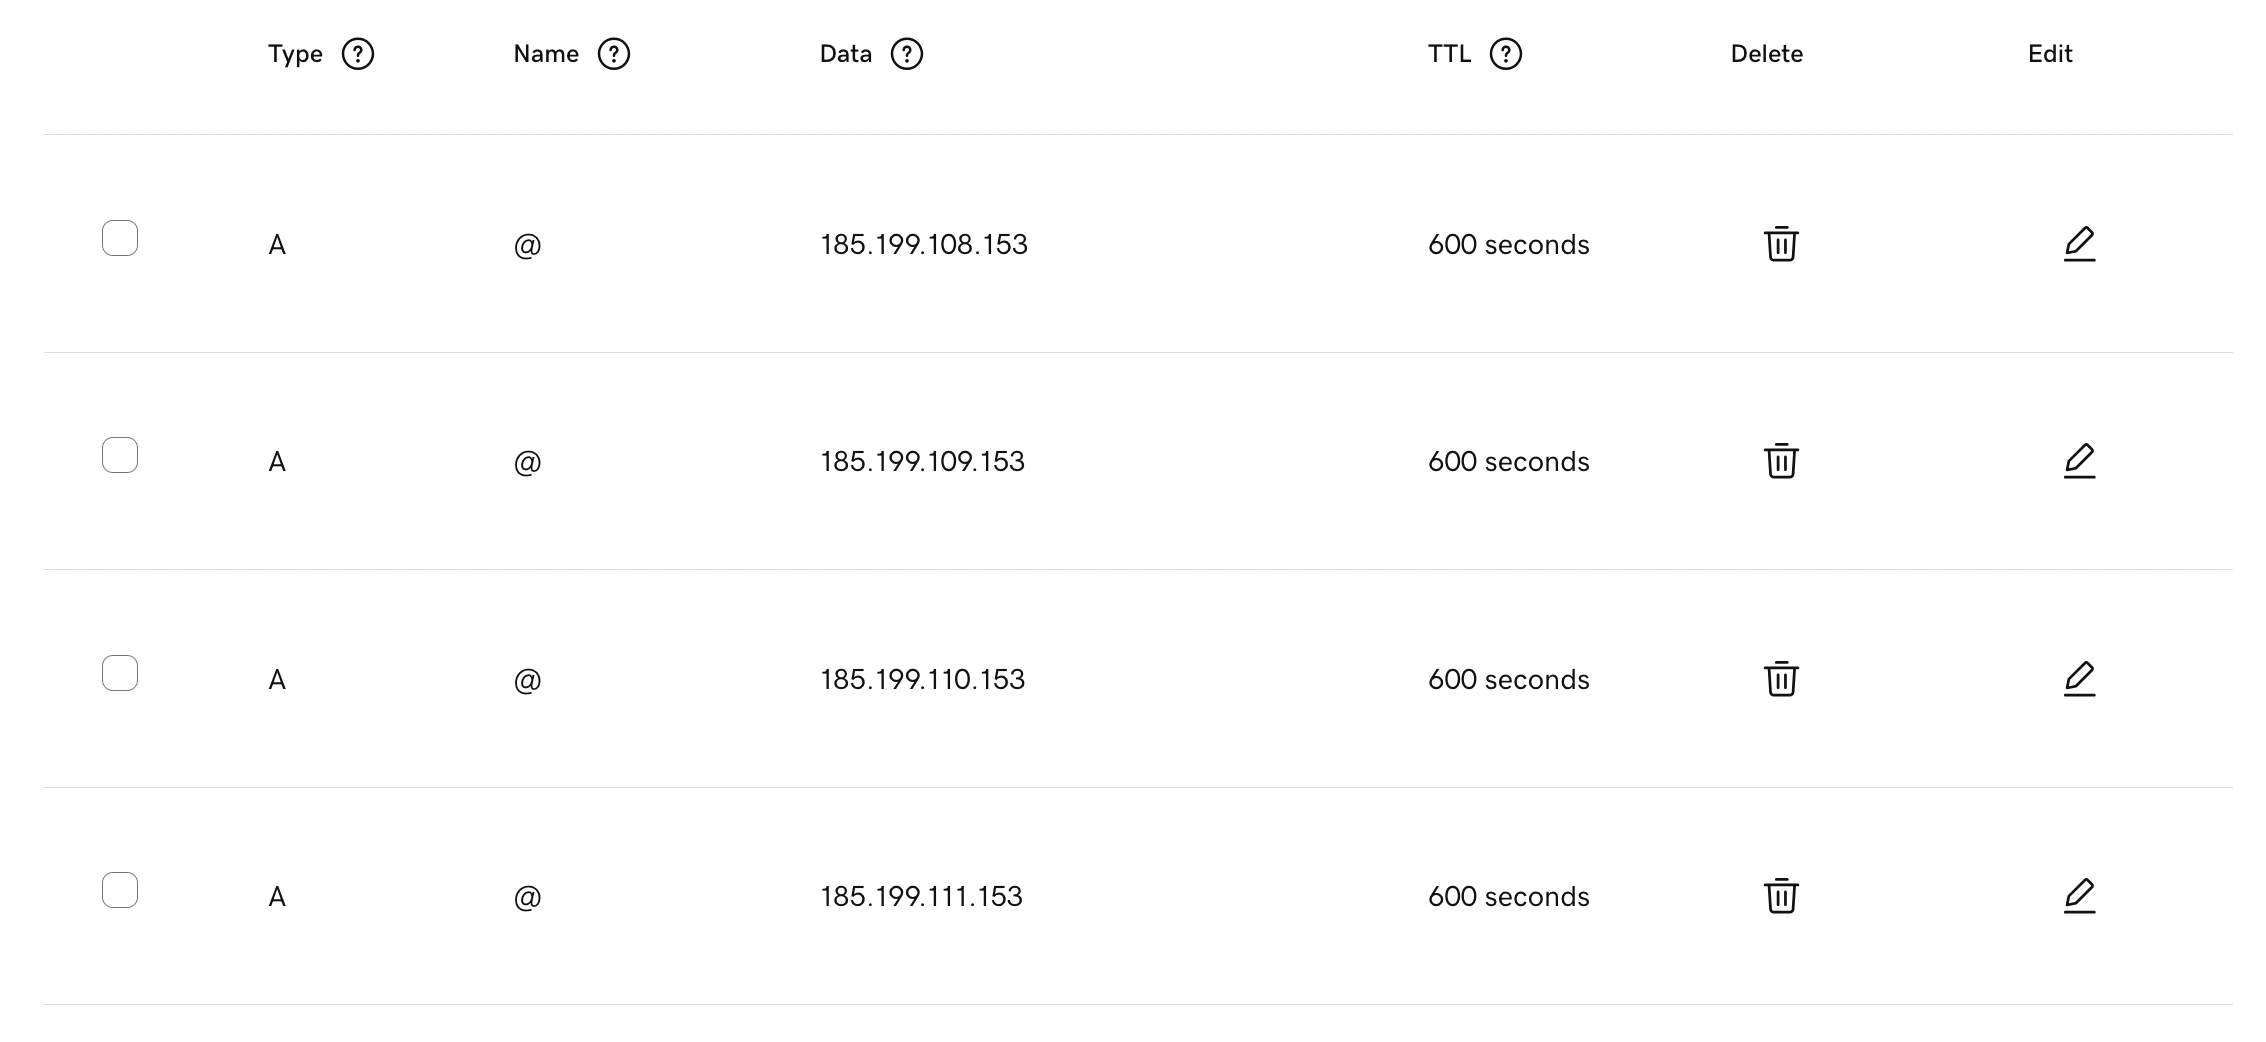
\includegraphics[width=1\linewidth,height=\textheight,keepaspectratio]{a-records.png}

\includegraphics[width=1\linewidth,height=\textheight,keepaspectratio]{cname-record.png}

All this is available from Domain/DNS/DNS Records at the \texttt{mobilebaydsa.org} control page in Godaddy; a more in-depth tutorial is available at \href{https://medium.com/@nbblks/how-to-set-up-godaddy-domain-with-github-pages-eaa65f88a8ec}{this Medium page}. Part of the original process involved also deleting the DNS records for the fallback site generated by Godaddy.

Github makes things easy to set up on its end: we publish the site to Github as a repository (\url{https://github.com/alabenian/mobilebaydsa}), enable Github Pages, which will automatically deploy it to \texttt{{[}username{]}.github.io/{[}repository\ name{]}}, then tell it to use the domain name \texttt{mobilebaydsa.org} and enforce HTTPS:

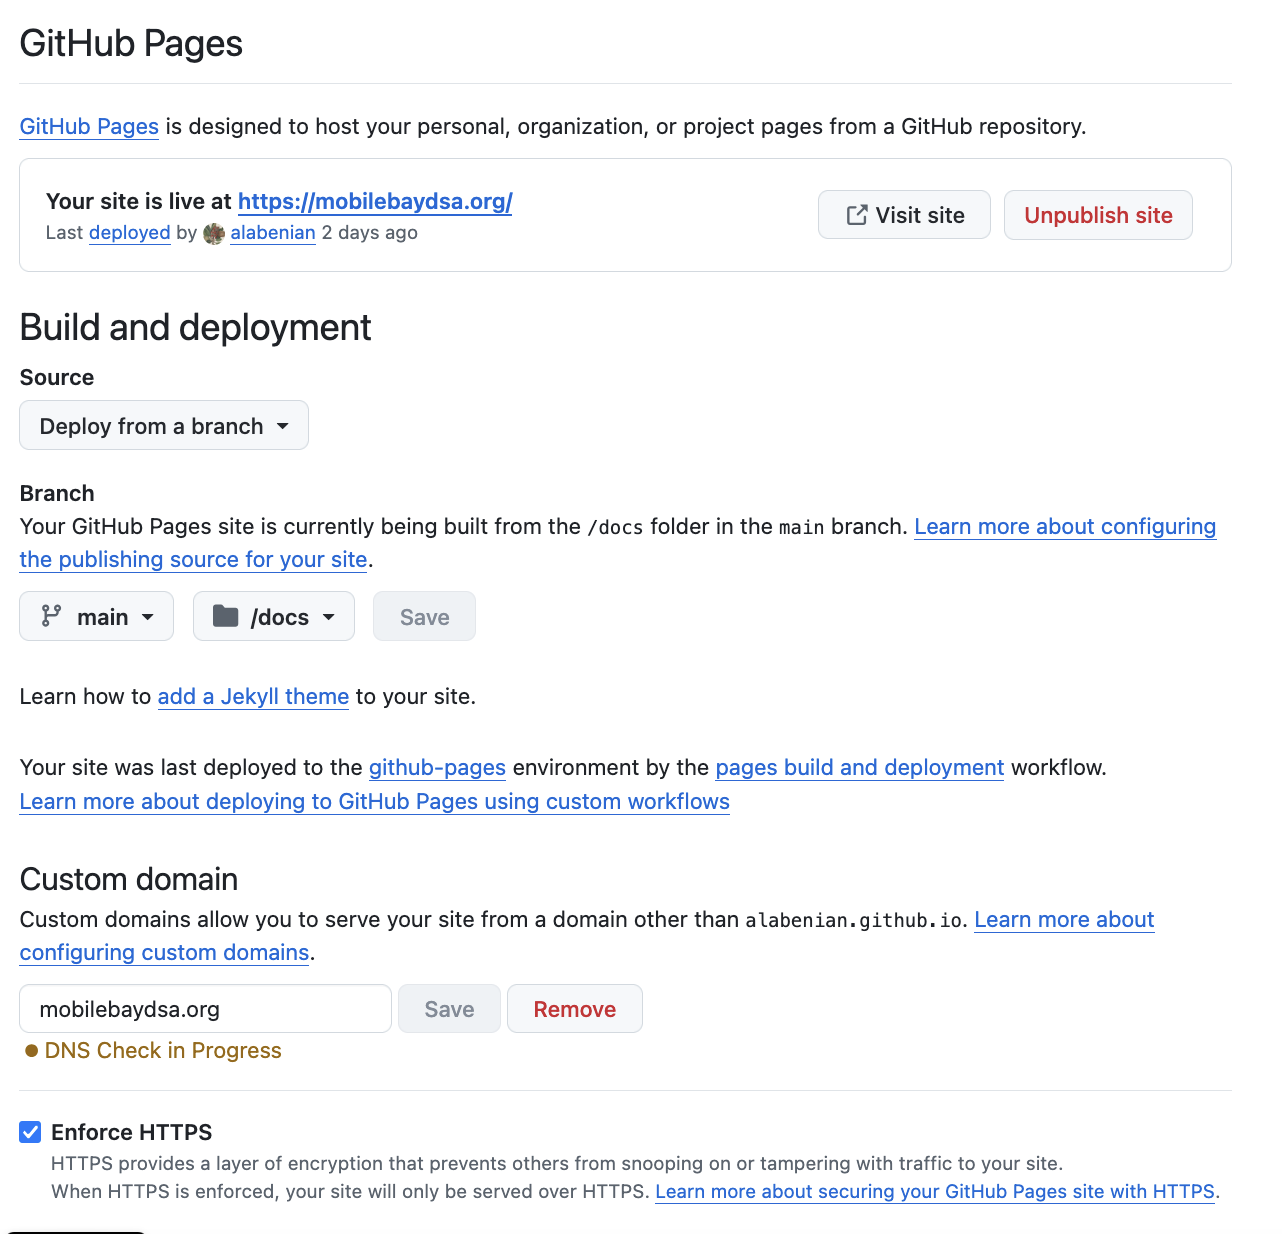
\includegraphics[width=0.75\linewidth,height=\textheight,keepaspectratio]{github-pages.png}

This should then automatically add a \texttt{CNAME} document containing ``\texttt{mobilebaydsa.org}'' to the repository. The only other setting I've changed here is to have it deploy from the \texttt{/docs/} folder of the repository rather than the root. Here \texttt{/docs/} is just a renamed version of the \texttt{/\_site/} output of Jekyll; this is deployed as a static site pre-built by Jekyll locally rather than one where Github runs Jekyll itself after changes are made to the repository, due to an incompatibility with one of the plugins I was using for our events posts (jekyll-leaflet). \emph{I will explain this more later, but for now, it's not relevant.}

\section{Github Pages and Potential Alternatives}\label{github-pages-and-potential-alternatives}

Github Pages is a nice, free choice of hosting which gives us maximal control over the website as mentioned before, but it can be somewhat daunting and even inaccessible to anyone who isn't already used to working with websites this way. The biggest con besides this is the fact that, on the free plan, all contents of the site have to be public unless an external service is used to store private, member-only information. Despite the extra difficulty of getting set up for those who would already have access, it's arguably more democratic than any other hosting service -- changes are published to the site when someone makes changes on their own download of the repository and sends them to Github through a \textbf{commit} with details of the changes they made to a local \textbf{branch} via the Github Desktop app (or via the command line), before making a \textbf{push request} that, when accepted, will publish them to the \textbf{main} branch and thereby the official website. The push request can be accepted by the owner (currently ``alabenian,'' but could be transferred to an official Mobile Bay DSA account) or anyone who has been listed as a collaborator on the project. This setup has the benefit of allowing \emph{anyone} to suggest changes to the website to be confirmed by authorized accounts. This way everyone has a voice to publish blog posts, new pages, design ideas, etc. to the site such that official collaborators can see every change and prevent security problems. I cited inaccessibility of editing as the main downside, but that's not too hard to get around either: with some effort I can make a separate service that allows for limited visual editing and makes automatic push requests for those changes.

One alternative would be a site builder like Wordpress.com which allows easier visual editing and supports blogs, etc. the same as Jekyll. Wordpress is especially nice because it would allow us to include member-only content on the website without a separate service, secured either by password or a whitelist of Wordpress accounts. Wordpress does not allow free sites to use custom domains, however, and the cheapest plan that \emph{does} is priced at \$96/year. Godaddy has a forwarding feature that would let us send anyone at \texttt{mobilebaydsa.org} to the Wordpress site, though I don't know how this would affect the site's presence in Google searches. The other major differences to consider are restrictions on design (which can also be removed with a \$24/year custom CSS add-on) and a Wordpress watermark that comes with the free plan (I've seen this on other DSA chapter sites, and it's not \emph{too} bad).

\part{Basic Structure \& Working on the Repository}\label{part-basic-structure-working-on-the-repository}

\chapter{Basic Setup}\label{basic-setup}

\section{Getting Started}\label{getting-started}

If you want to make changes to the repository, you'll first need to establish a local branch to work on. I'm writing this guide under the assumption that you've \emph{never} used Github before, in which case I'd recommend working through Github Desktop and Visual Studio Code. After downloading those apps, open Github Desktop, set up a Github account and follow the app's instructions to clone the repository into whatever directory you'd like using its link \url{https://github.com/alabenian/mobilebaydsa}. Then open the folder with Visual Studio Code, and install the following command-line tools in your terminal (either as a standalone ``command prompt'' window or from the bottom terminal tab in VSCode).

There are three command-line tools in total used to build the site: \textbf{Jekyll}, \textbf{Tailwind}, and \textbf{Markwhen}. Installing Jekyll takes the greatest priority, as it is necessary to build the site at all (if we switched to having Github build the site with Jekyll itself, installing it locally wouldn't be 100\% necessary, but it's still nice to be able to view what you've done before publishing). Tailwind is second, because it creates the \texttt{.css} file used by the rest of the site for styling. Because this file has already been created, Tailwind is only necessary for \emph{editing} it. Finally, Markwhen is only used to render and update the timeline used on the Calendar page of the site, and is only necessary to someone who is adding or removing events on the calendar.

\textbf{Jekyll} (\url{https://jekyllrb.com/}) simplifies work on the site by structuring the files by root directory markdown (or HTML) files containing the contents of each page, \texttt{\_layout} HTML files which are referenced in each to determine how the contents are presented, and \texttt{\_include} HTML files which are referenced in either the layout or content files to display some extra piece of the website (e.g.~a navbar or a commonly-occurring button or icon). The resulting file structure of the site will be discussed further in ``Repository Structure.'' It requires Ruby (\href{https://www.ruby-lang.org/en/documentation/installation/}{installation information here}) and RubyGems (which should be included with Ruby) to install via \texttt{gem\ install\ bundler\ jekyll} in the terminal. After installation, the site can be built by opening the repository folder in the terminal (or \texttt{cd}-ing into it; this is already done if you've opened the entire folder in VSCode, so you can use the terminal tab at the bottom) and running \texttt{bundle\ exec\ jekyll\ serve}. I've used some additional plugins on the site, so it'll throw an error on the first build and prompt you to install those; from there any work with Jekyll should be smooth sailing!

\textbf{Tailwind} (\url{https://tailwindcss.com/}) simplifies writing CSS for the site by supplying a set of classes with short and easy-to-remember names. It can be installed as a CLI tool with \texttt{npm\ install\ tailwindcss\ @tailwindcss/cli}. (This uses \texttt{npm}, so unfortunately you'll need to install Node first: \url{https://docs.npmjs.com/downloading-and-installing-node-js-and-npm}) To use it on the site, just open the folder in another terminal tab (or, again, \texttt{cd} into it) and run \texttt{npx\ @tailwindcss/cli\ -i\ ./styles/initstyles.css\ -o\ ./styles/finalstyles.css\ -\/-watch}. It will then replace the ``\texttt{@import\ "tailwindcss";}'' in the initial styles file and watch for future changes to re-run the command in that terminal instance. This adds so much extra hassle for getting set up to edit styles, I may remove it in the future -- it made the process of designing the site much easier for me because I had already installed it globally and knew its classes.

\textbf{Markwhen} renders the markwhen file \texttt{calendar\_source/main\_calendar.mw} into \texttt{calendar\_source/timeline.html}, which is embedded on the Calendar page. Install it using \texttt{npm\ i\ -g\ @markwhen/mw} (this also requires Node -- see instructions for Tailwind). After installation, all you need to do is run \texttt{mw\ calendar\_source/main\_calendar.mw\ calendar\_source/timeline.html} to update the timeline if changes to \texttt{main\_calendar.mw} have been made. See the ``Events \& Posts'' chapter for more information about editing the timeline.

\subsection{TLDR (``Just give me the instructions already!'')}\label{tldr-just-give-me-the-instructions-already}

\begin{enumerate}
\def\labelenumi{\arabic{enumi}.}
\tightlist
\item
  Create a Github account
\item
  Download and install Github Desktop and Visual Studio Code
\item
  Open Github Desktop and follow the instructions to log in and clone a repository. Use the link \texttt{https://github.com/alabenian/mobilebaydsa} or \texttt{alabenian/mobilebaydsa}.
\item
  Open Visual Studio Code, and within it, open the folder you created by cloning the repository in the previous step. Tell VSCode that you trust the author, then find the ``terminal'' tab at the bottom of the window.
\item
  (Windows) Download and install a Ruby release from \url{https://rubyinstaller.org/downloads/}.
\item
  (Mac) Use Homebrew (if you don't already have it installed, first run \texttt{/bin/bash\ -c\ "\$(curl\ -fsSL\ https://raw.githubusercontent.com/Homebrew/install/HEAD/install.sh)"}) to update your Mac's built-in installation of Ruby: \texttt{brew\ update} and then \texttt{brew\ install\ ruby} in your VSCode terminal.
\item
  (Windows) Download and install a release of NVM Windows from \url{https://github.com/coreybutler/nvm-windows/releases}. Then run ``\texttt{nvm\ install\ latest} in your VSCode terminal.
\item
  (Mac) Run the NVM install script: \texttt{curl\ -o-\ https://raw.githubusercontent.com/nvm-sh/nvm/v0.40.3/install.sh\ \textbar{}\ bash}
\item
  Still in your VSCode terminal, run these commands:
\end{enumerate}

\begin{itemize}
\tightlist
\item
  \texttt{gem\ install\ bundler\ jekyll}
\item
  \texttt{npm\ install\ tailwindcss\ @tailwindcss/cli}
\item
  \texttt{npm\ install\ @markwhen/mw}
\end{itemize}

\begin{enumerate}
\def\labelenumi{\arabic{enumi}.}
\setcounter{enumi}{7}
\tightlist
\item
  Mouse over to the ``+'' button to the right of the terminal and click it twice to create two more terminal tabs. In each of the tabs now open, run one of the following commands:
\end{enumerate}

\begin{itemize}
\tightlist
\item
  \texttt{bundle\ exec\ jekyll\ serve} -- This will prompt you to install some additional plugins. Afterwards, it will build and serve your website to some localhost port. Take note of the ``server address'' it gives you immediately after this, open it in your browser, and bookmark it if necessary for future reference to see the effects of your changes.
\item
  \texttt{npx\ @tailwindcss/cli\ -i\ styles/initstyles.css\ -o\ styles/finalstyles.css\ -\/-watch} -- This will add any Tailwind classes used throughout the website to the base stylesheet, generating finalstyles.css, which is used as the main stylesheet for the whole website.
\item
  \texttt{mw\ calendar\_source/main\_calendar.mw\ calendar\_source/timeline.html} -- This will re-render the timeline used on the Calendar page, which has not yet been edited. Adding or removing events is as simple as editing \texttt{calendar\_source/main\_calendar.mw} and then re-running this command, though I'd like it to be standard practice to create an event post complete with a map of the location to which each event on the timeline may link.
\end{itemize}

\begin{enumerate}
\def\labelenumi{\arabic{enumi}.}
\setcounter{enumi}{8}
\tightlist
\item
  Start working!
\end{enumerate}

\bibliography{book.bib,packages.bib}

\end{document}
